%!TEX root = ../paper.tex

% Hardly any difference between estimators
One of the most striking observations from \cref{s:results} is that the difference in performance between the two estimators is minimal.

	% Study differences further mbe vs sambe plot
		% Single Sphere Sets
		Plotting the densities estimated by \sambe as a function of those estimated by \mbe shows no interesting differences between the two estimators for data set \ferdosiOne through \baakmanFive.
		% Multi Sphere Sets
		However for data set \ferdosiTwo through \baakmanThree these plots reveal some differences between the estimators. As can be seen in \cref{fig:discussion:performance:two:mbevssambe}, using shape-adaptive kernels results in estimated densities that are generally higher than those estimated with a fixed-shape kernel for data set \ferdosiTwo and \baakmanTwo. Reviewing the raw data shows that \sambe underestimates densities less than \mbe on points near the mean of `Trivariate Gaussian 1'. The kernels in this neighborhood are all slightly anisotropic, which has allowed the shape-adaptive estimator to use more data points, to better approximate the local densities. Thus showing that estimating densities with shape-adaptive kernels can be advantageous.
		%
		\begin{figure}
			\centering
			\begin{subfigure}{0.3\textwidth}
				\centering
				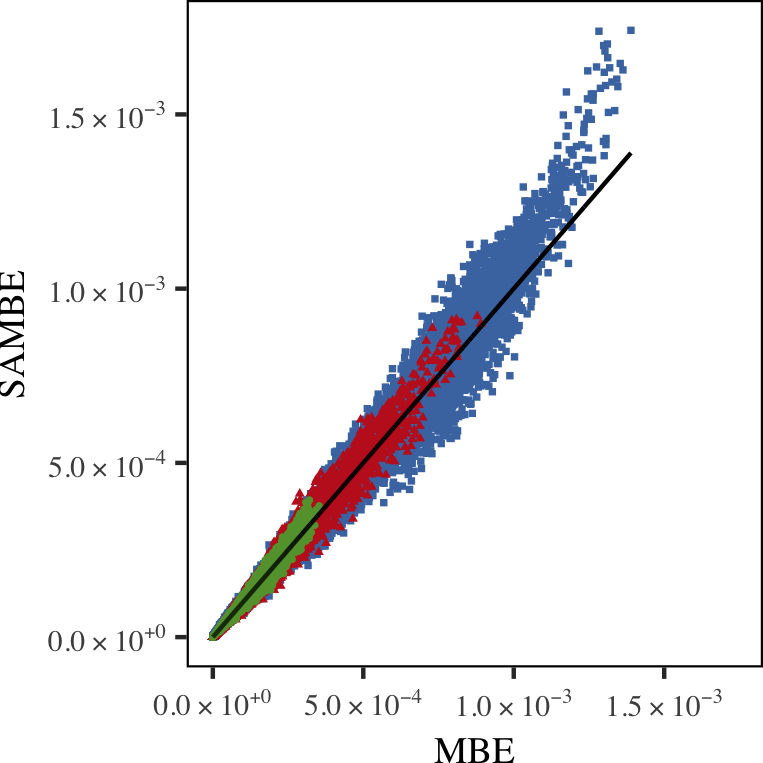
\includegraphics[keepaspectratio=true, width=\textwidth, height=0.23\textheight]{discussion/img/ferdosi_2_60000_mbe_sambe.png}
				\caption{Data set \ferdosiTwo}
				\label{fig:discussion:performance:mbevssambe:ferdosi2}
			\end{subfigure}
			\subfigvspace
			\begin{subfigure}{0.3\textwidth}
				\centering
				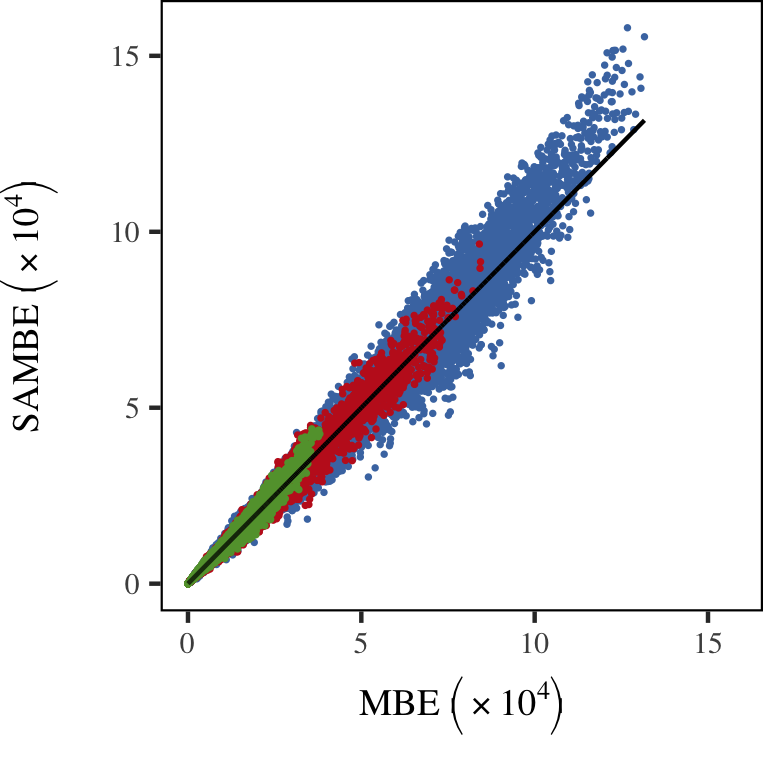
\includegraphics[keepaspectratio=true, width=\textwidth, height=0.23\textheight]{discussion/img/baakman_2_60000_mbe_sambe.png}
				\caption{Data set \baakmanTwo}
				\label{fig:discussion:performance:mbevssambe:baakman2}
			\end{subfigure}
			\caption{Plots of the densities estimated by \sambe as a function of those estimated by \mbe for data set %
				\subref{fig:discussion:performance:mbevssambe:ferdosi2} %
				\ferdosiTwo and %
				\subref{fig:discussion:performance:mbevssambe:baakman2} %
				\baakmanTwo.
			}
			\label{fig:discussion:performance:two:mbevssambe}
		\end{figure}

		% Ferdosi 3 / Baakman 3
		\Cref{fig:discussion:performance:four:mbevssambe} shows the opposite effect; the densities estimated by \sambe for data set \ferdosiThree and \baakmanThree are generally lower than those estimated by \mbe. Reviewing the raw data shows that the points where the differences in estimated densities between the two estimators are largest lie near the mean of the `Trivariate Gaussian 3' in both data set \ferdosiThree and \baakmanThree. The number of points used in the density estimate by \sambe is consistently lower than the number of points used by the fixed-shape estimator. Given the relatively high anisotropy of the kernels in that area we expect that this is due to the kernels reflecting fine local structures, instead of the global neighborhood.
		%
		\begin{figure}
			\centering
			\begin{subfigure}{0.3\textwidth}
				\centering
				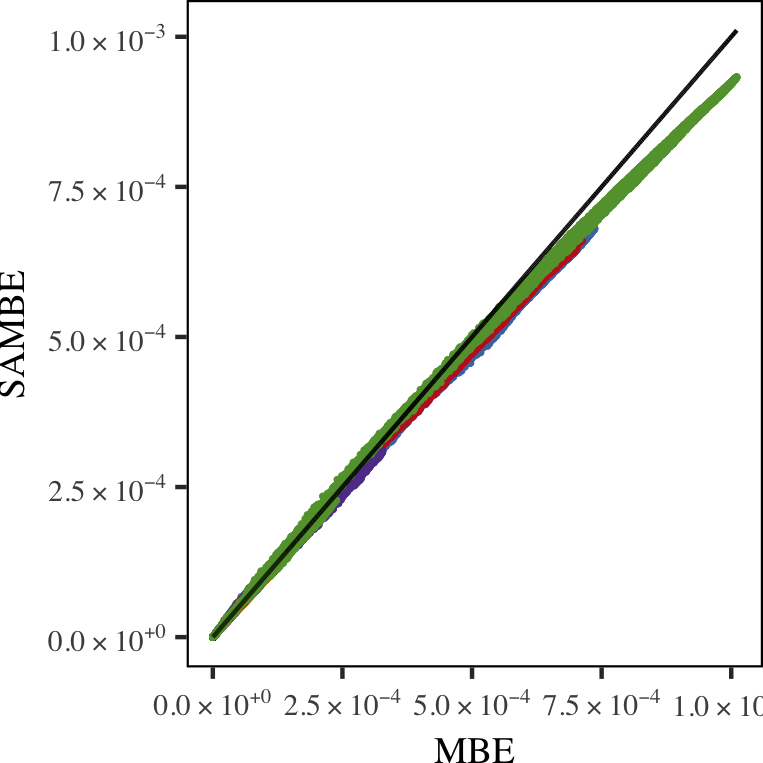
\includegraphics[keepaspectratio=true, width=\textwidth, height=0.23\textheight]{discussion/img/ferdosi_3_120000_mbe_sambe.png}
				\caption{Data set \ferdosiThree}
				\label{fig:discussion:performance:mbevssambe:ferdosi3}
			\end{subfigure}
			\subfigvspace
			\begin{subfigure}{0.3\textwidth}
				\centering
				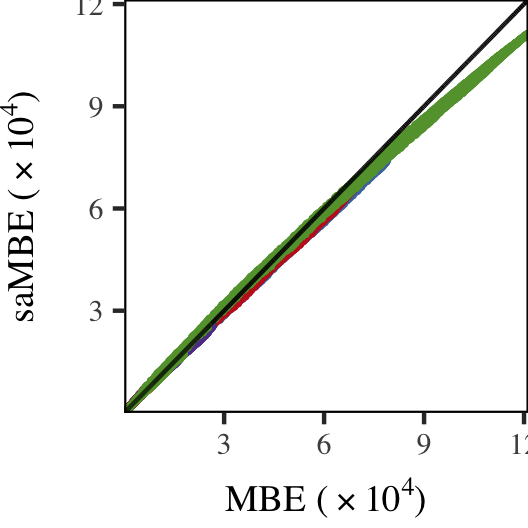
\includegraphics[keepaspectratio=true, width=\textwidth, height=0.23\textheight]{discussion/img/baakman_3_120000_mbe_sambe.png}
				\caption{Data set \baakmanThree}
				\label{fig:discussion:performance:mbevssambe:baakman3}
			\end{subfigure}
			\caption{Plots of the density estimated by \sambe as a function of those estimated by \mbe for data set %
				\subref{fig:discussion:performance:mbevssambe:ferdosi3} %
				\ferdosiThree and %
				\subref{fig:discussion:performance:mbevssambe:baakman3} %
				\baakmanThree.
			}
			\label{fig:discussion:performance:four:mbevssambe}
		\end{figure}

	% Where are the differences largest -> plots
	% Single Sphere
		\begin{figure}
			\centering
			\begin{subfigure}{0.23\textwidth}
				\centering
				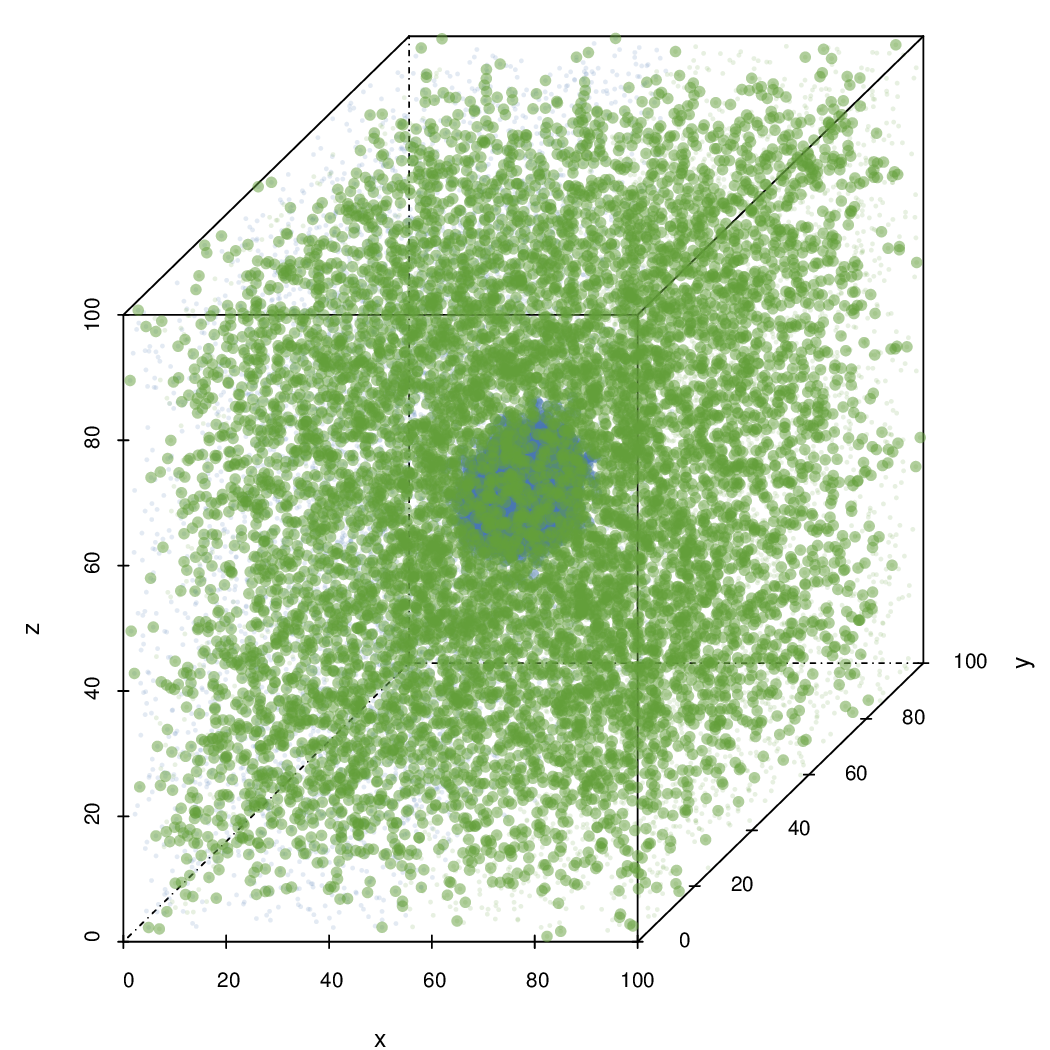
\includegraphics[keepaspectratio=true, width=\textwidth, height=0.23\textheight]{discussion/img/ferdosi_1_abs_error_mbeSmallerThansambe}
				\caption{Data set \ferdosiOne}
				\label{fig:discussion:performance:mbeLowerError:ferdosi1}
			\end{subfigure}
			\begin{subfigure}{0.23\textwidth}
				\centering
				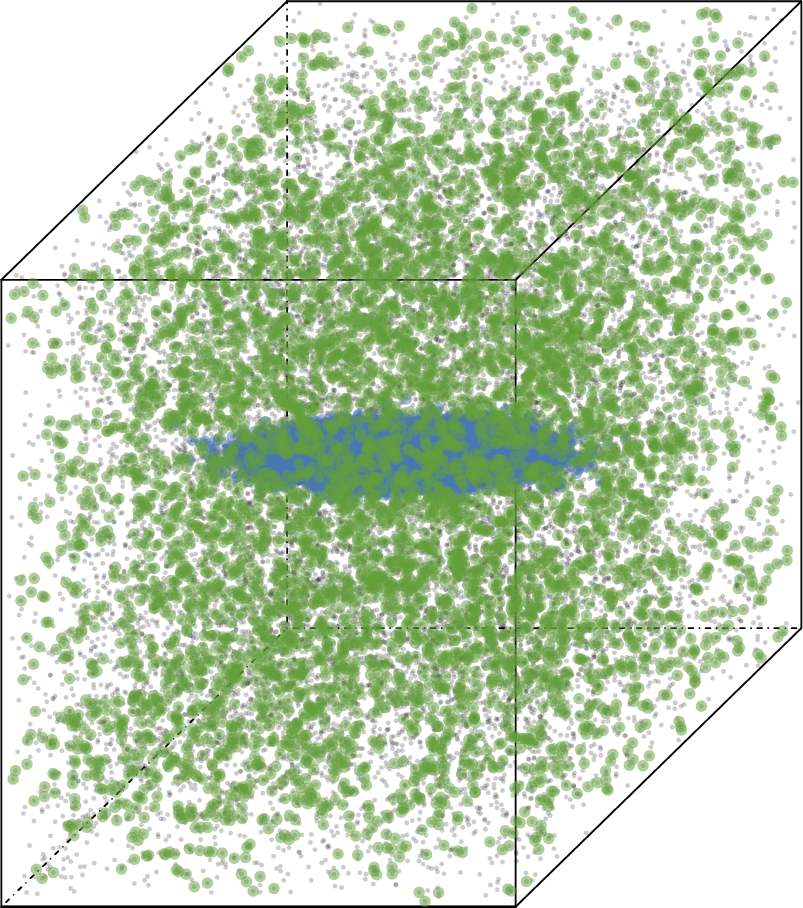
\includegraphics[keepaspectratio=true, width=\textwidth, height=0.23\textheight]{discussion/img/baakman_1_abs_error_mbeSmallerThansambe}
				\caption{Data set \baakmanOne}
				\label{fig:discussion:performance:mbeLowerError:baakman1}
			\end{subfigure}
			\subfigvspace
			\begin{subfigure}{0.23\textwidth}
				\centering
				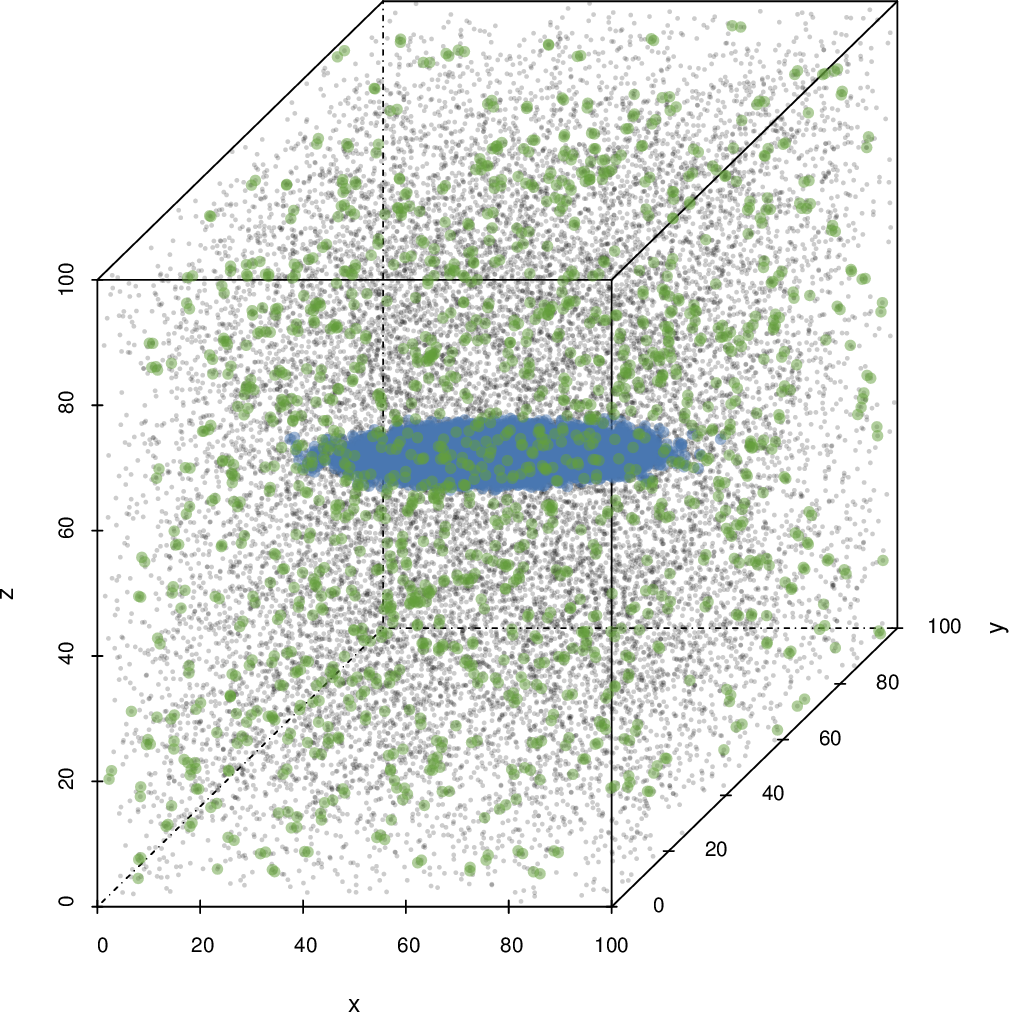
\includegraphics[keepaspectratio=true, width=\textwidth, height=0.23\textheight]{discussion/img/baakman_4_abs_error_mbeSmallerThansambe}
				\caption{Data set \baakmanFour}
				\label{fig:discussion:performance:mbeLowerError:baakman4}
			\end{subfigure}
			\begin{subfigure}{0.23\textwidth}
				\centering
				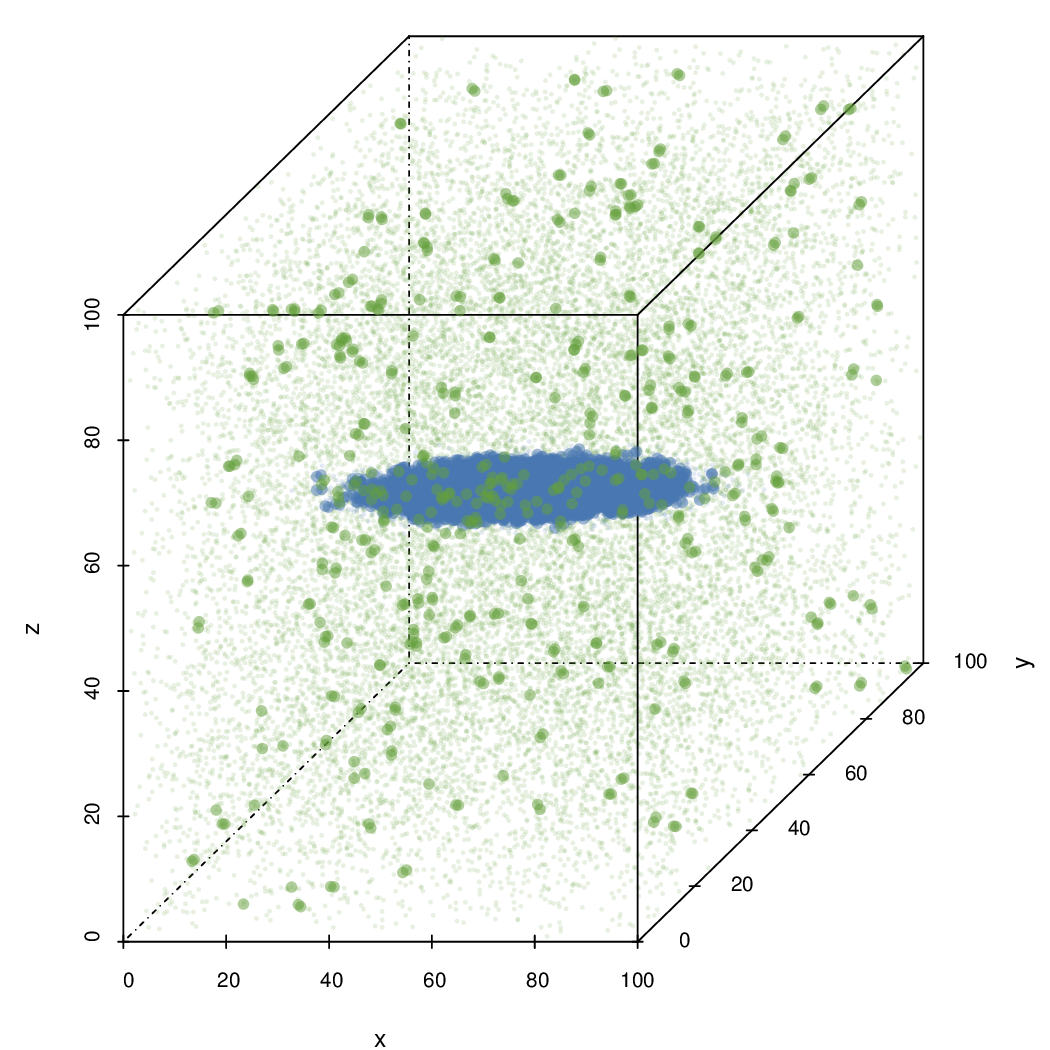
\includegraphics[keepaspectratio=true, width=\textwidth, height=0.23\textheight]{discussion/img/baakman_5_abs_error_mbeSmallerThansambe}
				\caption{Data set \baakmanFive}
				\label{fig:discussion:performance:mbeLowerError:baakman5}
			\end{subfigure}
			\caption{Low opacity scatter plot of set %
				\subref{fig:discussion:performance:mbeLowerError:ferdosi1} \ferdosiOne, %
				\subref{fig:discussion:performance:mbeLowerError:baakman1} \baakmanOne, %
				\subref{fig:discussion:performance:mbeLowerError:baakman4} \baakmanFour, and %
				\subref{fig:discussion:performance:mbeLowerError:baakman5} \baakmanFive, %
				with an overlay of larger, colored points where the absolute error of \sambe is greater than or equal to that of \mbe.}
			\label{fig:discussion:performance:singleSphere:mbeLowerError}
		\end{figure}
		%
		The plots in \cref{fig:discussion:performance:singleSphere:mbeLowerError} emphasize the points in data set \ferdosiOne and \baakmanOne where the absolute error of \mbe is smaller than that of \sambe. These plots show that the shape-adaptive kernels outperform symmetric kernels near the borders of the data sets.
			% Why the boundary effect
			We expect that this boundary effect is due to the strong anisotropy of the local neighborhood of the points near the limits of the data sets. Consequently the domain of the shape-adaptive kernels extends less outside of the boundaries of the data set than the domains of the symmetric kernels. This results in less underestimation of densities near the boundary of the data set, if shape-adaptive kernels are used.
			% Why is it stonger of the Gaussian is more anisotropic
			Furthermore the strength of the boundary effect seems to increase as the Gaussian component of the data set is more anisotropic. However the seemingly better performance of \sambe is due to an increase in the number of points where the density estimated by \sambe equals the density estimated by \mbe. In data set \ferdosiOne the two estimators give a different result on all points. The estimators agree on the density of \percentage{1.327294605254362e+01} of the points in data set \baakmanOne, this increases to \percentage{3.535329901731399e+01} in data set \baakmanFive.
			%SAMBE == MBE
			%Ferdosi 1 (0.000000000000000e+00 percent)
			%Baakman 1 (1.327294605254362e+01 percent)
			%Baakman 4 (2.989838892974129e+01 percent)
			%Baakman 5 (3.535329901731399e+01 percent)
			As the Gaussian component becomes more anisotropic the number of points whose local neighborhood consists only of points sampled from the uniform random background increases. On average the covariance matrix of neighborhoods that contain primarily points sampled from the background component should be scalar. Consequently as the anisotropy of the Gaussian component increases more shape-adaptive kernels take on a shape that is near-symmetric. This results in points were both estimators give the same approximated density.

	% Multi Sphere
		\begin{figure}
			\centering
			\begin{subfigure}{0.23\textwidth}
				\centering
				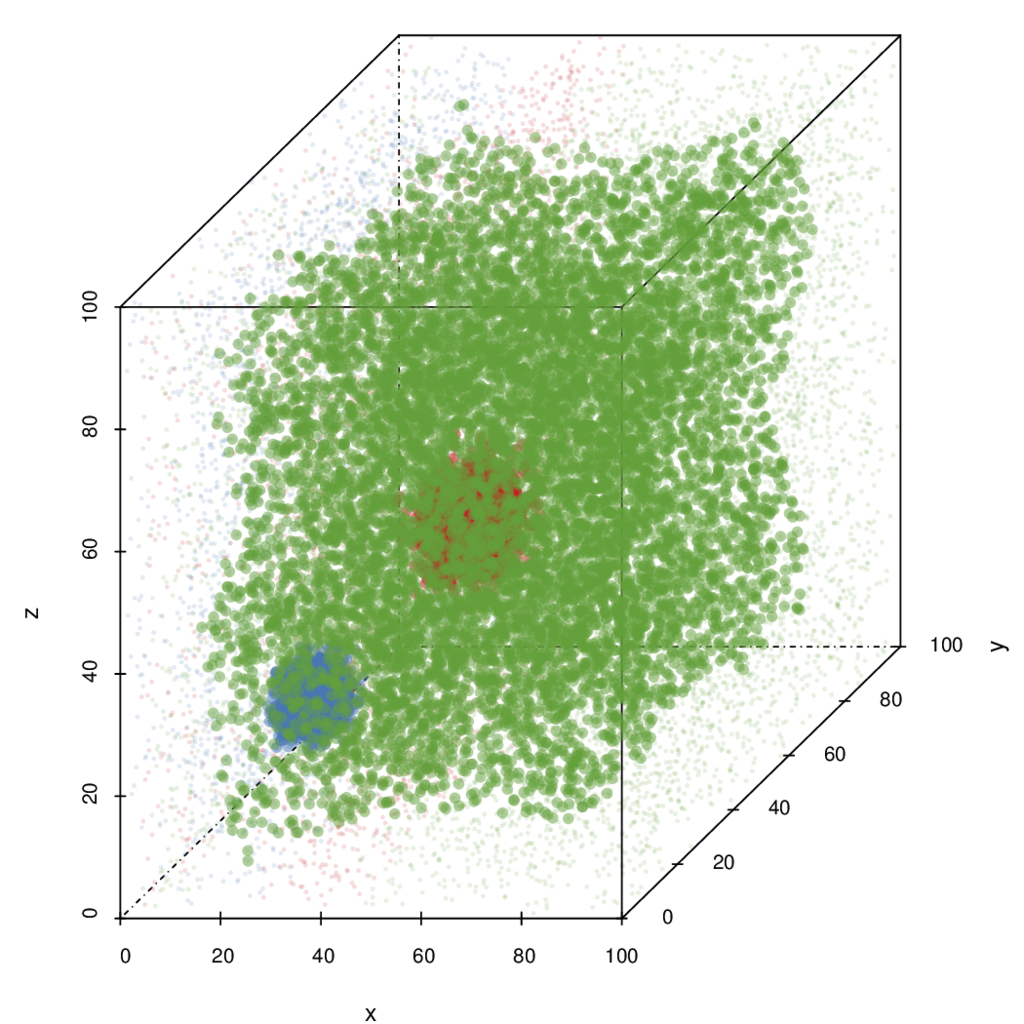
\includegraphics[keepaspectratio=true, width=\textwidth, height=0.23\textheight]{discussion/img/ferdosi_2_abs_error_mbeSmallerThansambe}
				\caption{Data set \ferdosiTwo}
				\label{fig:discussion:performance:mbeLowerError:ferdosi2}
			\end{subfigure}
			\begin{subfigure}{0.23\textwidth}
				\centering
				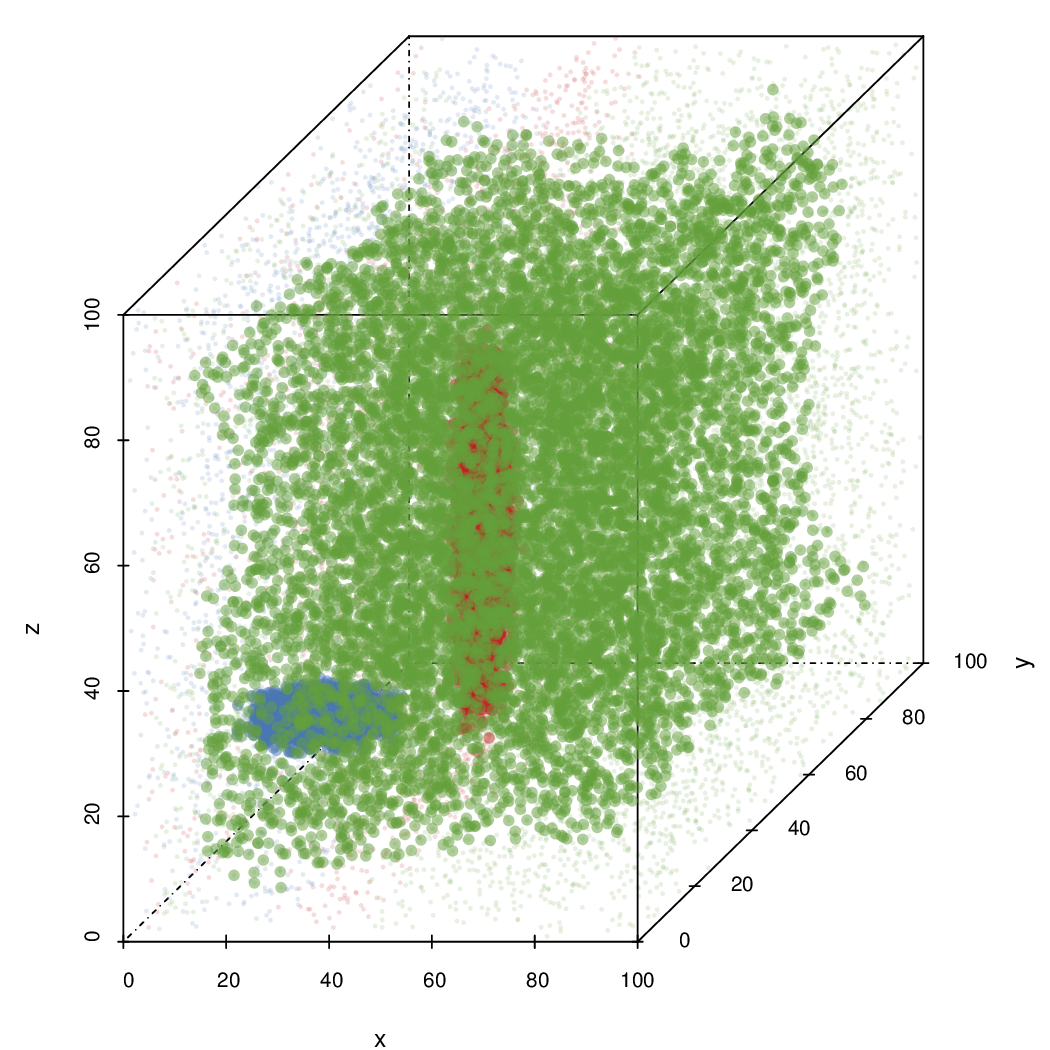
\includegraphics[keepaspectratio=true, width=\textwidth, height=0.23\textheight]{discussion/img/baakman_2_abs_error_mbeSmallerThansambe}
				\caption{Data set \baakmanTwo}
				\label{fig:discussion:performance:mbeLowerError:baakman2}
			\end{subfigure}
			\subfigvspace
			\begin{subfigure}{0.23\textwidth}
				\centering
				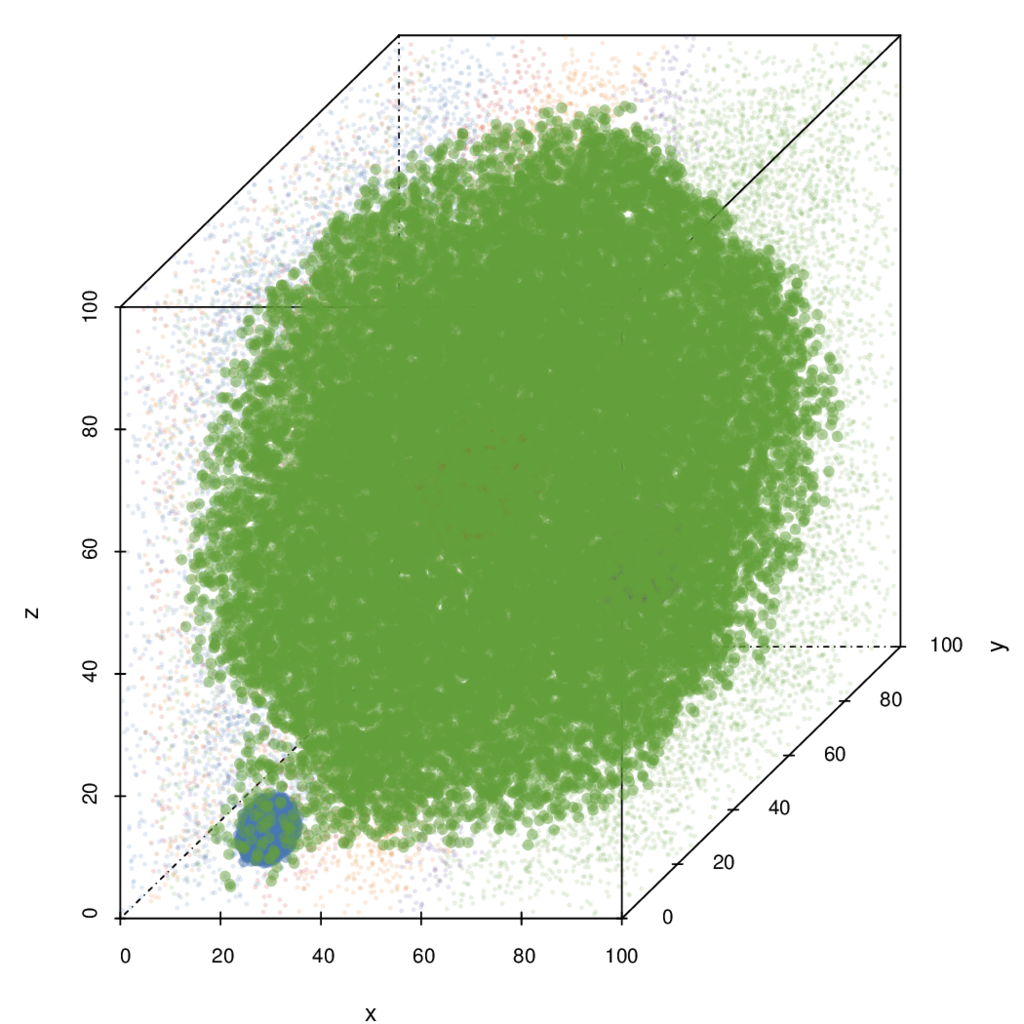
\includegraphics[keepaspectratio=true, width=\textwidth, height=0.23\textheight]{discussion/img/ferdosi_3_abs_error_mbeSmallerThansambe}
				\caption{Data set \ferdosiThree}
				\label{fig:discussion:performance:mbeLowerError:ferdosi3}
			\end{subfigure}
			\begin{subfigure}{0.23\textwidth}
				\centering
				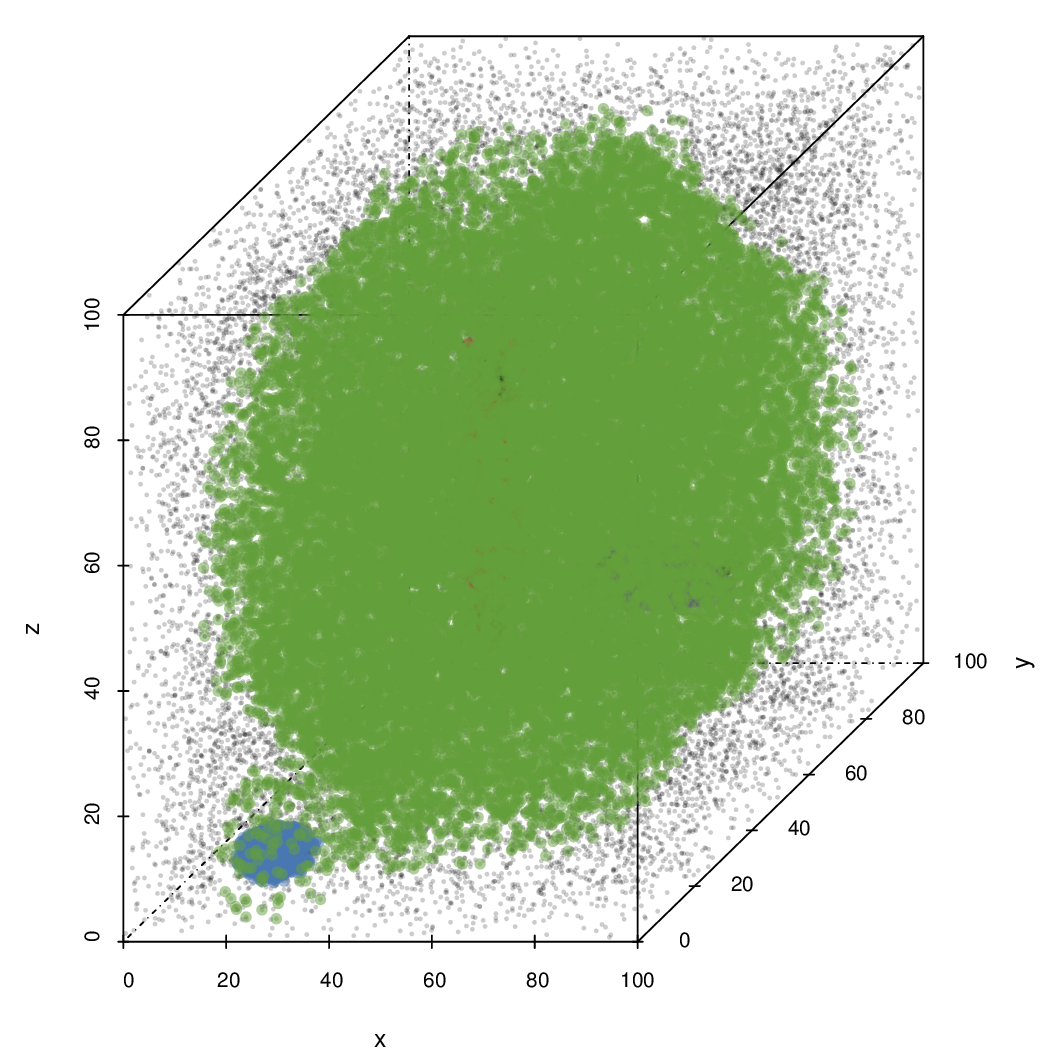
\includegraphics[keepaspectratio=true, width=\textwidth, height=0.23\textheight]{discussion/img/baakman_3_abs_error_mbeSmallerThansambe}
				\caption{Data set \baakmanThree}
				\label{fig:discussion:performance:mbeLowerError:baakman3}
			\end{subfigure}
			\caption{Low opacity scatter plot of data set %
				\subref{fig:discussion:performance:mbeLowerError:ferdosi2} \ferdosiTwo, %
				\subref{fig:discussion:performance:mbeLowerError:baakman2} \baakmanTwo, %
				\subref{fig:discussion:performance:mbeLowerError:ferdosi3} \ferdosiThree, and %
				\subref{fig:discussion:performance:mbeLowerError:baakman3} \baakmanThree %
				with an overlay of high opacity, larger points where the absolute error of \mbe is smaller than that of \sambe.}
			\label{fig:discussion:performance:multisphere:mbeLowerError}
		\end{figure}
		The points where using fixed-shape kernels results in a smaller error in data sets \ferdosiTwo through \baakmanThree are emphasized in
		\cref{fig:discussion:performance:multisphere:mbeLowerError}. We contribute the boundary effect in these data sets to the same cause as the boundary effect in the data sets with a single Gaussian component. Interestingly the points in data set \ferdosiThree and \baakmanThree where the absolute error of \mbe is lower, approximate a sphere, contrary to the cube they define for data set \ferdosiTwo and \baakmanTwo. It is our expectation that this is caused by the smaller distance between the means of the Gaussian components and the boundaries of the uniform random background in \ferdosiThree and \baakmanThree.
			% Define Ferdosi 3 Noise
			To test this we define data set \ferdosiThreeNoise, which replaces the uniform random background of \ferdosiThree with $\uniformDist{[-20, -20, -20]}{[120, 120, 120]}$. We adjust the number of points sampled from this component to ensure that its density is equal to that of the background component used in \ferdosiThree.
			% Is there any effect on the MSE
			The overall \mse of both estimators is slightly smaller for data set \ferdosiThreeNoise than for \ferdosiThree, however the \mse of `Trivariate Gaussian 1' and 3 shows a small increase.
			% Did the distance to the boundaries explain it?
			\Cref{fig:discussion:ferdosi3Noise:mbeLowerError} confirms that the spherical shape in \cref{fig:discussion:performance:mbeLowerError:ferdosi3,fig:discussion:performance:mbeLowerError:baakman3} is caused by the Gaussian near the boundary of the data set. As the shape defined by the emphasized points is now a cubical instead of spherical.
			% The Plots of Ferdosi 3 Noise
			\begin{figure}[b!]
				\centering
				\begin{subfigure}{0.23\textwidth}
					\centering
					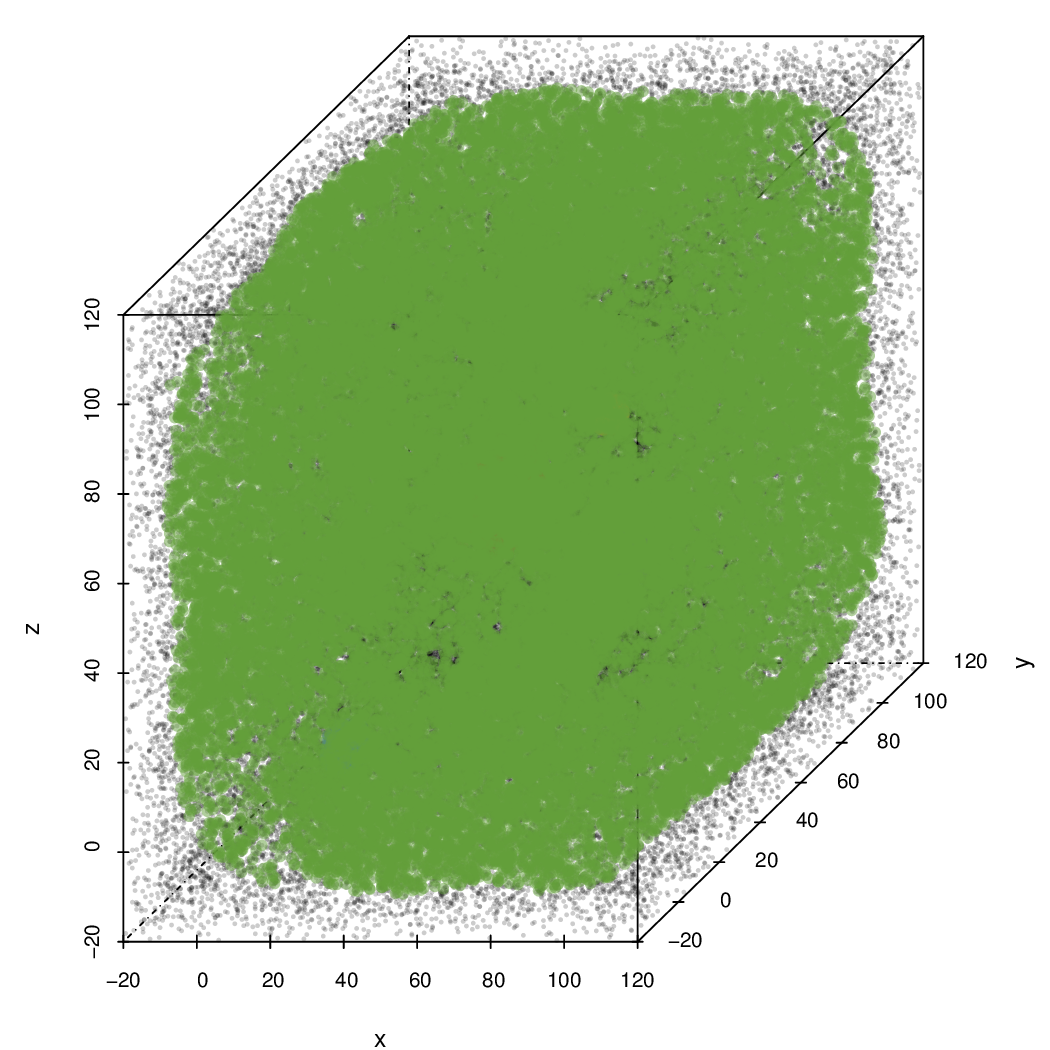
\includegraphics[keepaspectratio=true, width=\textwidth, height=0.23\textheight]{discussion/img/ferdosi_3_more_noise_abs_error_mbeSmallerThansambe.png}
					\caption{Absolute Error}
					\label{fig:discussion:ferdosi3Noise:mbeLowerError}
				\end{subfigure}
				\begin{subfigure}{0.23\textwidth}
					\centering
					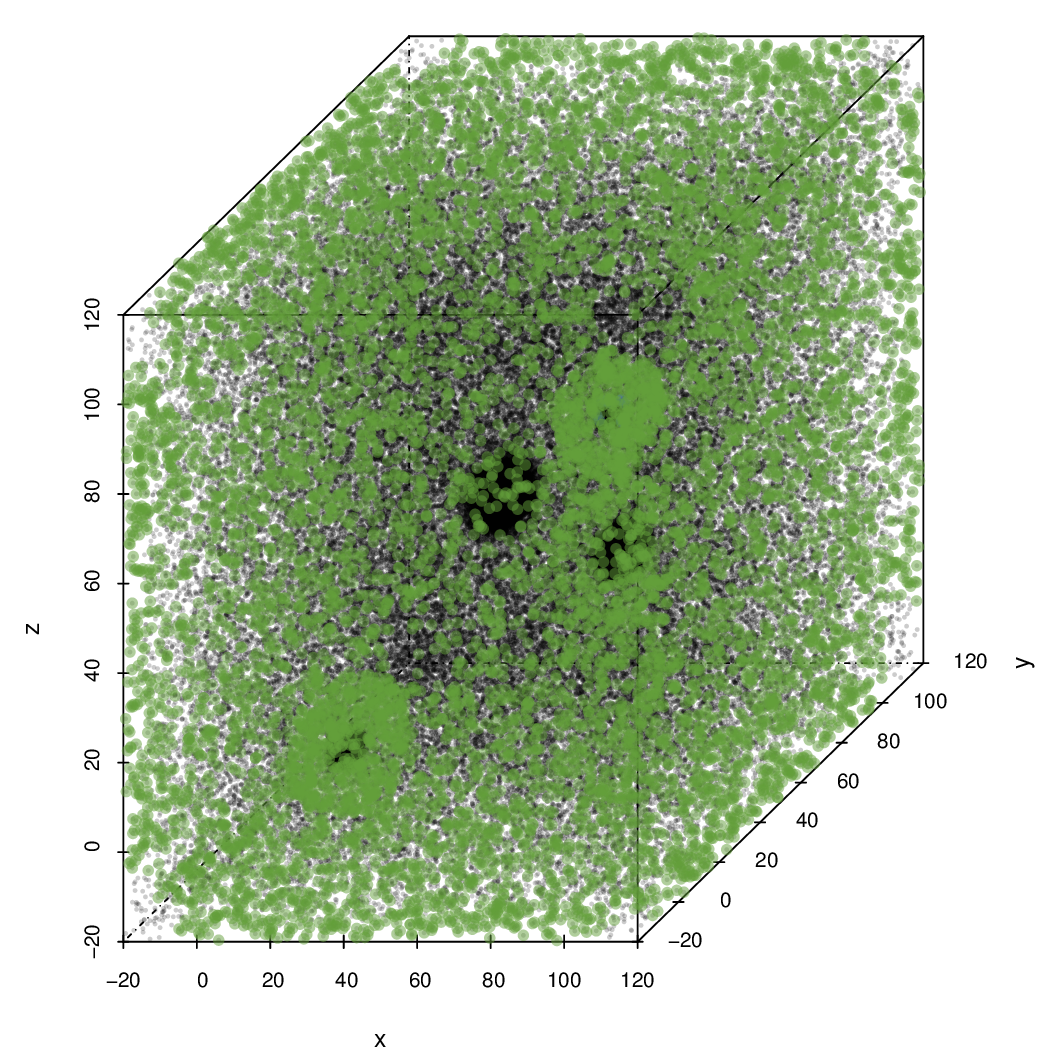
\includegraphics[keepaspectratio=true, width=\textwidth, height=0.23\textheight]{discussion/img/ferdosi_3_more_noise_anisotropy.png}
					\caption{Anisotropy}
					\label{fig:discussion:ferdosi3Noise:anisotropy}
				\end{subfigure}
				\caption{Low opacity scatter plot of data set \ferdosiThreeNoise with %
					\subref{fig:discussion:ferdosi3Noise:mbeLowerError} points where the absolute error of \mbe is lower than that of \sambe and %
					\subref{fig:discussion:ferdosi3Noise:anisotropy} points sampled from the Gaussian components with kernels whose anisotropy falls in the \nth{95} percentile of the complete data set emphasized.}
				\label{fig:discussion:ferdosi3Noise}
			\end{figure}

% Some conclusion
To conclude we have found that shape-adaptive kernels definitely improve performance in some cases, \ie near the boundary of the data sets and near the mean of some Gaussian components. Unfortunately in other cases the anisotropic kernels are detrimental. The difference in \mse between the two estimators shows that generally, using fixed-shape kernels is slightly advantageous.